\documentclass[a4paper, 12pt]{article}

% Sprache
\usepackage[ngerman]{babel}

% Pakete
\usepackage[utf8]{inputenc}
% lmodern, falls vorhanden (sonst Standard Computer Modern)
\IfFileExists{lmodern.sty}{\usepackage{lmodern}}{}
\usepackage{amsmath}
\usepackage{amssymb}
\usepackage{geometry}
\usepackage{fancyhdr}
\usepackage{graphicx}
\usepackage{subcaption}
\usepackage{hyperref}
\usepackage{booktabs}
\usepackage{tabularx}
\usepackage{titlesec}

\setlength{\parindent}{0pt}
\setlength{\parskip}{0.6em}
\geometry{a4paper, margin=1in, headsep=35pt}

% Weniger Abstand ober- und unterhalb der Section-Überschriften
\titlespacing*{\section}{0pt}{0.6ex plus .1ex minus .1ex}{0.2ex plus .1ex}

% Section-Überschriften eine Stufe kleiner (Large -> large)
\titleformat*{\section}{\large\bfseries}

% Lange \texttt-Bezeichner dürfen umbrechen
\sloppy

% Referenzen
\usepackage{csquotes}
\usepackage[style=verbose-ibid,backend=bibtex]{biblatex}

% Kopfzeile anpassen
\pagestyle{fancy}
\fancyhead{}
\fancyhead[L]{\veranstaltung}
\fancyhead[C]{\textbf{Jan-Niclas Loosen}\\ \textbf{Mat.Nr. UNKENNTLICH}}
\fancyhead[R]{Universität Trier\\ \today}

% Variablen für Anpassungen
\newcommand{\veranstaltung}{Het. Computing\\ Übungsblatt 2}
\bibliography{references.bib}

% Automatisch aus results/*.json erzeugte Messwerte und Geräte-Flags.
% Erzeugung: python -m gpubench values  (bzw. ./run_all.sh).
\IfFileExists{values.tex}{% Auto-generated from results/*.json by gpubench.report_values.
% Do not edit by hand; run `python -m gpubench values` (or run_all.sh).
\newif\ifdevicegpu
\devicegpufalse
\newcommand{\bwCoalesced}{48{,}1}
\newcommand{\bwGather}{9{,}0}
\newcommand{\bwPeakCopy}{40{,}8}
\newcommand{\bwRatio}{5{,}3}
\newcommand{\bwStrided}{11{,}6}
\newcommand{\computeUnits}{8}
\newcommand{\deviceName}{cpu-skylake-avx512-AMD Ryzen AI 9 HX PRO 370 w/ Radeon 890M}
\newcommand{\deviceType}{CPU}
\newcommand{\divDegHigh}{64}
\newcommand{\divFactor}{1{,}4}
\newcommand{\divHigh}{20{,}0}
\newcommand{\divLow}{14{,}2}
\newcommand{\globalMemGiB}{13{,}6}
\newcommand{\maxClock}{1996}
\newcommand{\maxWorkGroup}{4096}
\newcommand{\npGather}{1{,}1}
\newcommand{\npPeakGflops}{19{,}3}
\newcommand{\npStream}{7{,}7}
\newcommand{\occHigh}{48{,}3}
\newcommand{\occLow}{37{,}5}
\newcommand{\occWgHigh}{512}
\newcommand{\occWgLow}{8}
\newcommand{\peakGflops}{20{,}8}
\newcommand{\satN}{1{,}7 \cdot 10^{7}}
\newcommand{\smallGflops}{3{,}0}
\newcommand{\smallN}{1024}
\newcommand{\waveFront}{8}
}{%
  \newif\ifdevicegpu\devicegpufalse
  \newcommand{\deviceName}{(unbekannt, values.tex fehlt; \texttt{gpubench values} ausführen)}%
}

\begin{document}

\section*{Einführung}
Ziel dieser Übung ist es, das \textit{SIMT-Ausführungsmodell} (Single Instruction, Multiple Threads) einer GPU messbar und damit sichtbar zu machen. Dazu habe ich mit PyOpenCL\autocite{pyopencl} zwei Mikro-Benchmarks gebaut. Der erste nutzt einen rechenintensiven \textit{Kernel} (Funktion, die auf der GPU läuft) und vermisst den Durchsatz in \textit{GFLOP/s} (Anzahl Gleitkomma-Operationen pro Sekunde) über die Problemgröße sowie über den Grad der \textit{Warp-Divergenz} (Threads im selben Warp nehmen verschiedene Verzweigungen). Der zweite ist ein speicherintensiver Streaming-Kernel und untersucht die effektive Bandbreite für drei Zugriffsmuster sowie das Verbergen von Latenzen über die \textit{Occupancy} (Anteil der gleichzeitig aktiven Warps am Hardware-Maximum). Als Vergleichspunkt dient jeweils eine CPU-Referenz auf Basis von NumPy.

Die OpenCL-Kernels werden zur Laufzeit vom Treiber übersetzt\autocite{opencl} und auf der Hardware ausgeführt, während die gesamte Steuerung über Python erfolgt. Weil Numpy Matrizenoperationen hardware-optimiert in C bzw. C++ ausführt, sind auch die Vergleichsbenchmarks aussagkräftig. Die hier genannten Messungen wurden auf einer AMD Ryzen AI 9 HX PRO 370 CPU mit einer AMD Radeon 890M Graphics On-Board-GPU ausgeführt. Die implementierten Scripts sollten allerdings geräteunabhängig mit \texttt{python -m gpubench all} ausgeführt werden können.

Die folgenden Erklärungen beschreiben die hardwareseitigen SIMT-Mechanismen und ordnen die gemessenen Werte ein. Obwohl viele Begrifflichkeiten in den AMD nahen Dokumentationen anders sind (bspw. Warps vs. Wavefronts), hält sich dieses Dokument an die in der Vorlesung genutzten NVIDIA Namenskonventionen.

\section*{Aufbau und Messmethodik}
Ein \texttt{device}-Modul wählt einen OpenCL-Kontext (Organisationsstruktur um den Kernel) und liest zunächst die Geräteeigenschaften aus. Das für die Tests genutzte Gerät meldet \computeUnits{} Compute Units, eine maximale Work-Group-Größe von \maxWorkGroup{} und ein bevorzugtes Vielfaches der Work-Group-Größe von \waveFront{}. Dieses Vielfache nutze ich als Stellvertreter für die Warp-Breite (bei NVIDIA typischerweise $32$, auf AMD-GPUs $64$). Die Zeitmessung erfolgt über OpenCL-Profiling-Events, die ausschließlich die Kernel-Laufzeit auf dem Gerät erfassen und damit den Host-Overhead ausklammern. Jede Messung verwendet zwei Aufwärmläufe und meldet anschließend den Median aus mehreren Wiederholungen, um Einschwing- und Ausreißereffekte zu dämpfen. Alle Ergebnisse werden als JSON abgelegt.

\section*{Aufgabe 1: SIMT und Warp-Divergenz}
Im rechenintensiven Kernel bearbeitet jedes Work-Item genau ein Element und führt darauf eine feste Zahl von FMA-Schritten (Fused Multiply-Add: $x = x \cdot \mathrm{COEF} + \mathrm{BIAS}$) mit je zwei FLOPs je Schnritt aus. Abbildung~\ref{fig:scaling} zeigt den Durchsatz über der Problemgröße $n$. Bei kleinem $n$ ($\smallN$ Work-Items) liegt der Durchsatz mit $\smallGflops$~GFLOP/s niedrig, weil zu wenige Threads vorhanden sind, um die Recheneinheiten auszulasten und Startkosten zu amortisieren. Mit wachsendem $n$ steigt der Durchsatz und sättigt bei etwa $\peakGflops$~GFLOP/s (bei $n \approx \satN$). Auf einer GPU markiert dies den Übergang, ab dem alle Compute Units mit genügend Warps gefüllt sind, sodass sich SIMT lohnt.

\begin{figure}[h!]\centering
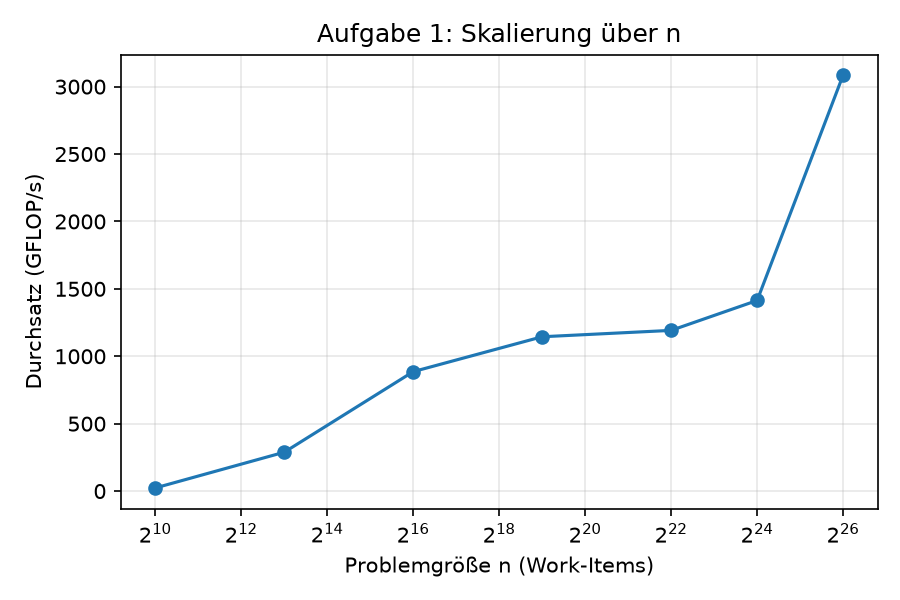
\includegraphics[width=0.75\textwidth]{figures/scaling.png}
\caption{Durchsatz über der Problemgröße $n$ (logarithmische $n$-Achse).}\label{fig:scaling}\end{figure}

Den Kern der Aufgabe bildet die Warp-Divergenz. Im divergenten Kernel wählt jedes Work-Item anhand von \texttt{get\_local\_id(0) \% DEGREE} einen von \texttt{DEGREE} Pfaden. Dabei leistet jeder Pfad exakt dieselbe Arbeit, sodass die Gesamtarbeit je Work-Item unabhängig vom Divergenzgrad konstant bleibt. Auf einer GPU führt ein Warp seine Lanes im Lockstep aus: Nehmen die Lanes unterschiedliche Verzweigungen, so arbeitet der Warp die \texttt{DEGREE} Pfade serialisiert nacheinander ab. In jedem Durchlauf ist nur die zu diesem Pfad gehörende Lane-Gruppe aktiv, während die übrigen Lanes maskiert mitlaufen und ihre Ergebnisse verworfen werden. Da jeder Durchlauf die volle Zeit kostet, fällt der Durchsatz annähernd auf $1/\mathrm{DEGREE}$. Abbildung~\ref{fig:divergence} zeigt die Messung und bestätigt die Theorie: Der Durchsatz sinkt von $\divHigh$~GFLOP/s (kein divergenter Pfad) auf $\divLow$~GFLOP/s bei Grad $\divDegHigh$, also um den Faktor $\divFactor$.

\begin{figure}[h!]\centering
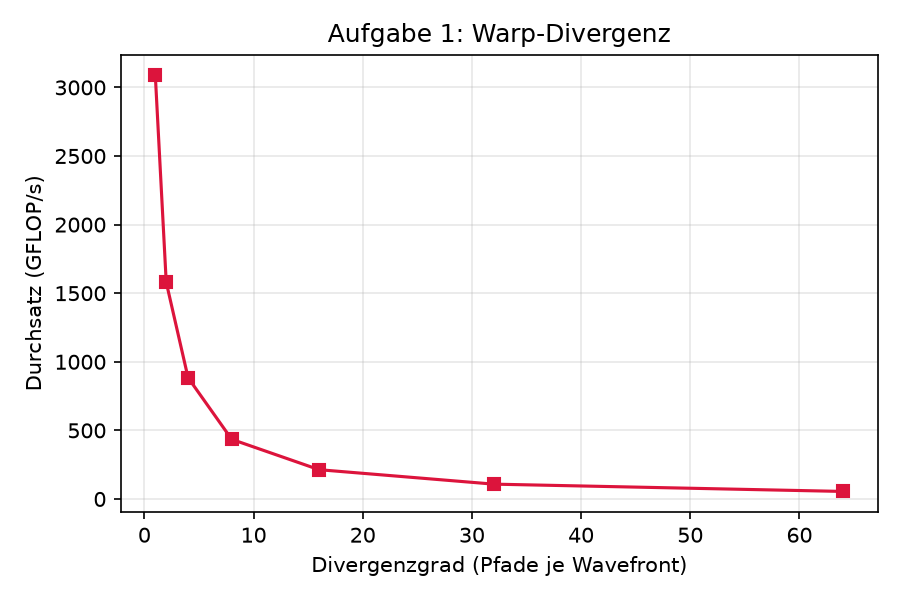
\includegraphics[width=0.75\textwidth]{figures/divergence.png}
\caption{Durchsatz über dem Divergenzgrad (Pfade je Warp).}\label{fig:divergence}\end{figure}

Dieser steile, annähernd mit $1/\mathrm{DEGREE}$ verlaufende Einbruch ist die unmittelbare Folge der Lockstep-Ausführung, die divergente Pfade serialisiert. Die NumPy-Referenz auf der CPU bleibt im Gegensatz dazu über die Divergenzgrade nahezu konstant, da ein CPU-Kern Sprungvorhersage und unabhängige Pfadausführung besitzt und beliebig viele Verzweigungen damit kaum kosten.

\section*{Aufgabe 2: Speicherzugriff und Latency-Hiding}
Der speicherintensive Kernel berechnet $b[i] = a[\mathrm{idx}[i]] \cdot c$ und besitzt eine sehr geringe arithmetische Intensität, ist also bandbreitenbegrenzt. Das Indexfeld \texttt{idx} kodiert das Zugriffsmuster, sodass ein einziger Kernel alle drei Muster fair vermisst: coalesced (Identität), strided (großer, zu $n$ teilerfremder Schritt) und gather (zufällige Permutation mit festem Seed). Abbildung~\ref{fig:patterns} zeigt die effektive Bandbreite. Der coalesced-Zugriff erreicht $\bwCoalesced$~GB/s und liegt damit nahe an der separat gemessenen Kopier-Spitzenbandbreite von $\bwPeakCopy$~GB/s. Der strided-Zugriff bricht auf $\bwStrided$~GB/s ein, der gather-Zugriff auf $\bwGather$~GB/s; coalesced ist somit rund um den Faktor $\bwRatio$ schneller als gather. Auf einer GPU verschmilzt die Hardware benachbarte Zugriffe eines Warps zu wenigen Speichertransaktionen (Coalescing). Unregelmäßige Adressen zerfallen dagegen in viele einzelne Transaktionen und lasten die Bandbreite schlecht aus.

\begin{figure}[h!]\centering
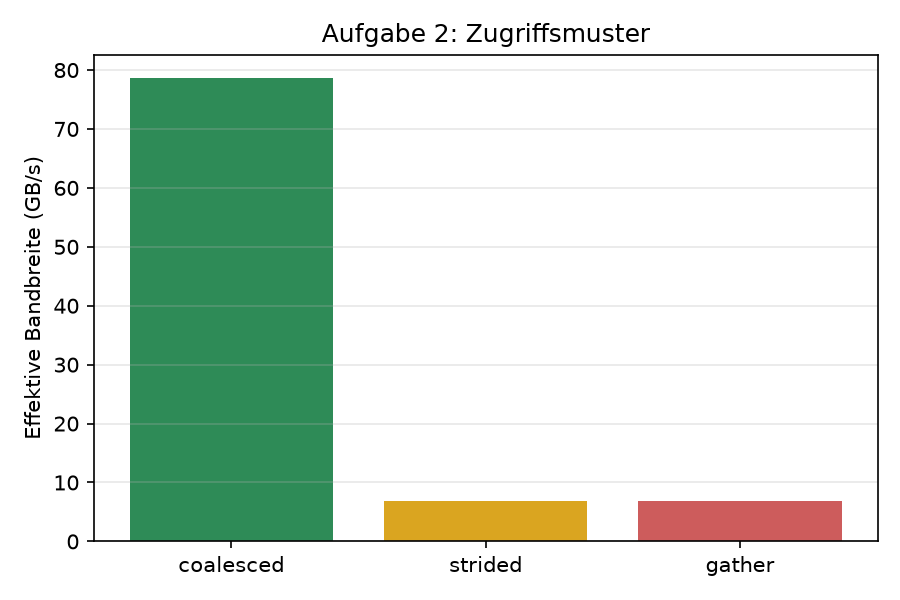
\includegraphics[width=0.75\textwidth]{figures/patterns.png}
\caption{Effektive Bandbreite je Zugriffsmuster.}\label{fig:patterns}\end{figure}

Abbildung~\ref{fig:occupancy} variiert die Work-Group-Größe und damit die Occupancy, also das Verhältnis aus aktiven zu maximal möglichen Warps je Compute Unit. Die Bandbreite steigt von $\occLow$~GB/s bei $\occWgLow$ Work-Items je Gruppe auf $\occHigh$~GB/s bei $\occWgHigh$ und läuft dann in ein Plateau. Die GPU verbirgt Speicherlatenz nicht über große Caches, sondern über massive Parallelität: Wartet ein Warp auf Daten, schaltet der Scheduler auf einen anderen lauffähigen Warp um. Erst wenn genügend Warps resident sind, wird die Latenz vollständig verdeckt. Die CPU verfolgt die entgegengesetzte Strategie und verbirgt Latenz über die Cache-Hierarchie und Prefetching: Die NumPy-Referenz erreicht sequenziell $\npStream$~GB/s, beim zufälligen gather aber nur $\npGather$~GB/s, weil dann nahezu jeder Zugriff einen Cache-Miss erzeugt.

\begin{figure}[h!]\centering
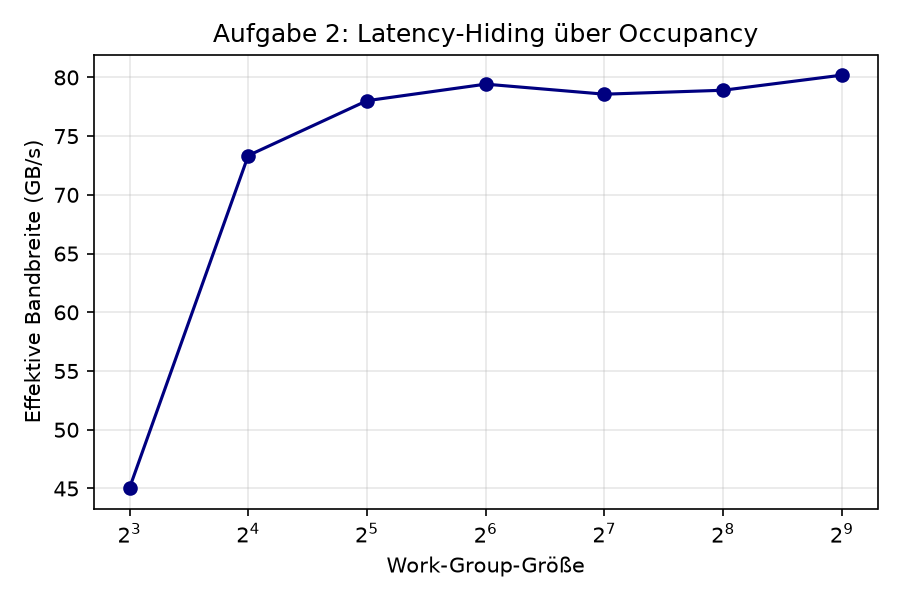
\includegraphics[width=0.75\textwidth]{figures/occupancy.png}
\caption{Bandbreite über der Work-Group-Größe (Occupancy).}\label{fig:occupancy}\end{figure}

\section*{Fazit}
Tabelle~\ref{tab:summary} fasst die Messungen zusammen.
\ifdevicegpu
Sie stellt die GPU \deviceName{} der NumPy-CPU-Referenz gegenüber.
\else
Sie stellt das OpenCL-Gerät (hier POCL-CPU) der NumPy-Referenz gegenüber; auf einer GPU erzeugt derselbe Ablauf die Gerätespalte neu.
\fi

\begin{table}[h]\centering
\begin{tabularx}{\textwidth}{l *{2}{>{\centering\arraybackslash}X}}
\toprule
\textbf{Messung} & \textbf{\ifdevicegpu GPU\else OpenCL (POCL-CPU)\fi} & \textbf{NumPy (CPU)} \\
\midrule
Spitzen-Durchsatz (GFLOP/s)            & $\peakGflops$ & $\npPeakGflops$ \\
Divergenz-Einbruch (Grad 1 zu \divDegHigh)  & Faktor $\divFactor$ & nahezu konstant \\
Bandbreite coalesced (GB/s)            & $\bwCoalesced$ & $\npStream$ \\
Bandbreite gather (GB/s)               & $\bwGather$ & $\npGather$ \\
\bottomrule
\end{tabularx}
\caption{Zusammenfassung der Messungen.}\label{tab:summary}\end{table}

Beide Experimente zeigen dieselbe Konsequenz des SIMT-Modells: Hoher Durchsatz entsteht nur bei divergenzarmen Kontrollflüssen und bei regelmäßigen, coalescten Datenlayouts. Wo eine CPU über Sprungvorhersage und Caches einzelne unregelmäßige Zugriffe abfedert, bestraft die GPU sie durch Serialisierung der Pfade und durch zerfallende Speichertransaktionen. Für GPU-Anwendungen folgt daraus unmittelbar, Datenstrukturen so anzuordnen, dass benachbarte Threads benachbarte Daten lesen, und Verzweigungen innerhalb eines Warps möglichst zu vermeiden.

\end{document}
